\documentclass[/home/greg/Thesis/main/main.tex]{subfiles}
\usepackage{floatrow}
\newfloatcommand{capbtabbox}{table}[][\FBwidth]
%\title{Neutron star mechanics in the observers inertial frame}
%\author{}

\begin{document}
\graphicspath{{/home/greg/Neutron_star_modelling/TimingResiduals/img/}}

\newcommand{\Phiexact}{\Phi_{\mathrm{exact}}}
\newcommand{\Phifit}{\Phi_{\mathrm{fit}}}
\newcommand{\wobbleangle}{\tilde{\theta}}
\FloatBarrier

\section{Timing residuals}
The principle observational quantifty reported on for a pulsar is the timing 
residual. This is measured by the difference between the TOA of a pulse and
a timing model of the pulsar. It is the quasi-periodic structure in
the timing residual which we term timing-noise and hence we naturually want 
to be able to calculate the residual from our analytic models.

Equation \eqref{eqn: Phi} gives the exact phase evolution of the star, we will
label this as $\Phiexact$. We then take a Taylor expansion to the phase
about some fixed time $t_{0}$
\begin{equation}
    \Phi(t; t_{0}, \phi, \f, \fdot, \fddot) = 
    \phi + 2\pi \left(\f(t - t_{0}) + 
                          \frac{\fdot}{2!}(t-t_{0})^{2} +
                          \frac{\fddot}{3!}(t-t_{0})^{3} 
                          \right),
\label{eqn: TR taylor expansion} 
\end{equation}
and use a least-squares fitting method to minimise the squared error between
the Taylor expansion and $\Phiexact$. The resulting coefficients 
$\{\phi_{0}, \f_{0}, \fdot_{0}, \fddot_{0}\}$ are the quantities best describing the
NS under a power law spindown; in pulsar astronomy these are refered to as 
the timing model. We will refer to the best-fit phase as described by  these
coeffients as
\begin{equation}
    \Phifit(t) = \Phi(t; t_{0}, \phi_{0}, \f_{0}, \fdot_{0}, \fddot_{0})
\end{equation}
The phase-residual is then defined as the difference between the exact phase 
and the fitted phase
\begin{equation}
  \Delta\Phi(t) = \Phiexact(t) - \Phifit(t).
\end{equation}
It is worth noting that a phase-residual depends on the fit to the entire
length of date provided in $\Phiexact$. The phase residual can be rescaled to
give the timing residual by calculating the residual as a fraction of a cycle
then multiplying by the period
\begin{equation}
    \Delta T = \frac{\Delta\Phi(t)}{2\pi} P.
    \label{eqn: phase to timing}
\end{equation}
Over a typical observation periods it is possible for the period to
fractionally change due to the spindown. For this work we will report only on
phase-residuals although to make contact with observational results we will
require this rescaling.

The effect of free-precession and the inclusion of a spin-down torque was
considered analytically by \citet{Jones2001}. This provides a set of useful
results with which to verify our simulations and the subsequent processing
required to calculate the timing residual. 

Before continuing we need to define the wobble angle $\wobbleangle$, this is the angle
between the spinvector and the axis about which it precesses. Without the EM
torque, this is the body-frame $\z$ axis defined as one of the principle axis
of the moment of inertia. In such a situation the wobble angle is simply given
by 
\begin{equation}
    \wobbleangle=\theta,
\end{equation}
as used in \citet{Jones2001}. 
Including the EM torque introduces two effects. The
first and the largest is the transformation induced by the anomalous torque
which causes the spin-vector to precess about the principle axis of the
effective body-frame. This has already been discussed in chapter \ref{sec:
effective body frame} and results in a wobble angle
\begin{equation}
    \wobbleangle = \theta - \beta
\end{equation}
where $\beta$ is the rotation from the body-frame to the effective body-frame. 
The second effect is that, even without the anomalous torque the spin-down 
torque rotates the axis about which the spin-vector precesses. This is a smaller
effect and can be shown to produce a wobble angle of the order $P/\tau_{s}$. 
This will always be significantly smaller than the other angles and so can be
neglected for now.

\subsection{Effect of free precession on the phase residual: geometric effect}
\citet{Jones2001} analysed the geometric effect that precession will have on
the timing residual. This was done by considering the motion of the magnetic
dipole in the inertial frame as the superposition of motions due to the fast
rotation period and the slow precession. The results
must be separated into two cases when $\theta > \chi$ and $\theta < \chi$. Of
these two the authors argue that `the wobble angle ($\theta$) of rapidly rotating
stars are to small values by the finite crustal breaking strain'. Therefore, 
the second case $\theta < \chi$ holds greater physical relevance and so we 
focus on this region of parameter space. The phase residual was found to be 
given by  
\begin{equation}
    \Delta\Phi^{49}(t) = -\wobbleangle \frac{\cos\chi}{\sin\chi}\cos(\dot{\psi t}),
    \label{eqn: Jones 49}
\end{equation}
where the superscript here refers to the equation number from \citet{Jones2001}.
For a freely precession star $\dot{\psi}=\epsI \f$ is the constant free
precession frequency. Therefore, the magnitude of variations is given by 
$|Delta\Phi^{49}|=\wobbleangle \cot(\chi)$. 

Equation \eqref{eqn: Jones 49} is calculated in the absence of any EM torque.
Nevertheless, it is still appropriate when such a torque is applied provided
that the geometric effect is stronger that any others(these are discussed in
the next few sections). As such we begin by simulating a NS with the properties
listed in table \ref{tab: 49 verification properties}. Unphysical values of the
rotation frequency and magnetic field have been used to aid the computational
speed. The resutlting phase residual, in cycles, is given in figure \ref{fig:
TR 49}.

%\begin{table}[ht]
    %\centering
    % \begin{tabular}{ccl}
\multicolumn{3}{c}{Simulation parameters} \\
\hline
$\omega_0$  &=& 15.5 rad/s\\
$B_0$  &=& $ 1.581\times 10^{14} $ G \\
$\chi$  &=& 49.99$^{\circ}$ \\
$a_0$ &=& 2.00$^{\circ}$ \\
$\tilde{\theta}$ &= & 2.04$^{\circ}$
\end{tabular}
    
    %\caption{}
    %\label{tab: 49 verification properties}
%\end{table}

%\begin{figure}[ht]
%\centering
	%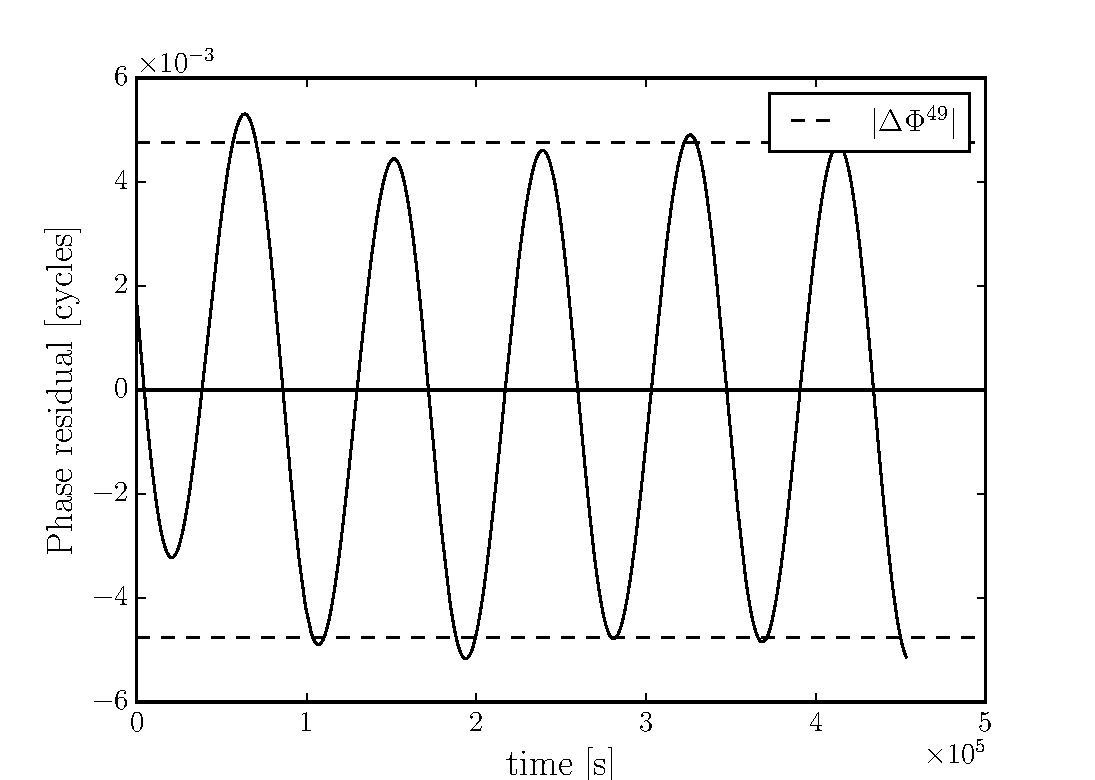
\includegraphics[width=0.7\textwidth]{49_verification.pdf}
%\caption{The phase residual in cycles for a simulated NS with the properties described in table \ref{tab: 49
%verification properties}. This is used to illustrate the agreement with the magnitude
%of variations from equation \eqref{eqn: Jones 49} taken from \citet{Jones2001}.}
%\label{fig: TR 49}
%\end{figure}

\begin{figure}[htb]
\begin{floatrow}
\ffigbox{%
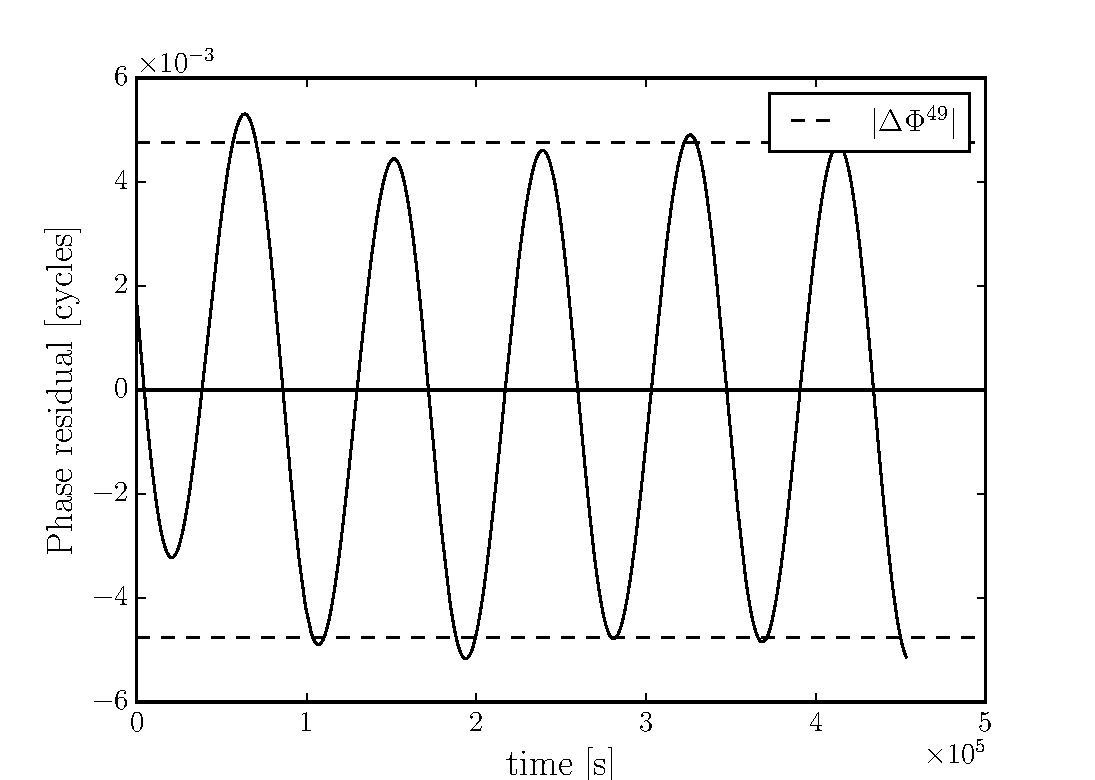
\includegraphics[width=0.5\textwidth]{49_verification.pdf}
}{%
  \caption{The phase residual in cycles for a simulated NS with the properties described in table \ref{tab: 49
verification properties}. This is used to illustrate the agreement with the magnitude
of variations from equation \eqref{eqn: Jones 49} taken from \citet{Jones2001}.}%
  \label{fig: PR 49}
}
\capbtabbox{%
   \begin{tabular}{ccl}
\multicolumn{3}{c}{Simulation parameters} \\
\hline
$\omega_0$  &=& 15.5 rad/s\\
$B_0$  &=& $ 1.581\times 10^{14} $ G \\
$\chi$  &=& 49.99$^{\circ}$ \\
$a_0$ &=& 2.00$^{\circ}$ \\
$\tilde{\theta}$ &= & 2.04$^{\circ}$
\end{tabular}
    
}{%
  \caption{}%
  \label{tab: 49 verification properties}
}
\end{floatrow}
\end{figure}

\FloatBarrier
\subsection{Effect of free precession on the phase residual: effect of the electromagnetic
torque}
Considering a vacuum point-dipole spin-down torque (like the one introduced in 
\ref{sec: defining the model}) \citet{Jones2001} found that the EM torque can
amplify the geometric effect of equation \eqref{eqn: Jones 49}. The magnitude
of variation due to EM torque is given by 
\begin{equation}
    |\Delta\Phi^{63}| = \frac{1}{\pi}\left(\frac{\tau_{P}}{P}\right)
    \left(\frac{\tau_{P}}{\tau_{S}}\right) 
                                    |\Delta\Phi^{49}|
\label{eqn: Jones 63}
\end{equation}
The two ratios of time-scales define an `amplification factor'. This effect is
important for young pulsars with short periods.

We simulate such a star using the properties in table \ref{tab: 63 verification
properties} noting that the amplification factor is $\sim 3$ when including the
factor of $\pi$. The resulting phase residual is plotted in figure \ref{fig: PR
63} along with the magnitude of variations due to free precession along and the
amplification due to the EM torque.

%\begin{table}[ht]
%    \centering
%     \begin{tabular}{ccl}
\multicolumn{3}{c}{Simulation parameters} \\
\hline
$\omega_0$  &=& 1550.0 rad/s\\
$B_0$  &=& $ 1.581\times 10^{14} $ G \\
$\chi$  &=& 49.99$^{\circ}$ \\
$a_0$ &=& 2.00$^{\circ}$ \\
$\tilde{\theta}$ &= & 2.06$^{\circ}$ \\
$\mathcal{A}_{\mathrm{EM}}$ &= & $41.0$
\end{tabular}
    
%    \caption{}
%    \label{tab: 63 verification properties}
%\end{table}
%
%\begin{figure}[ht]
%\centering
%	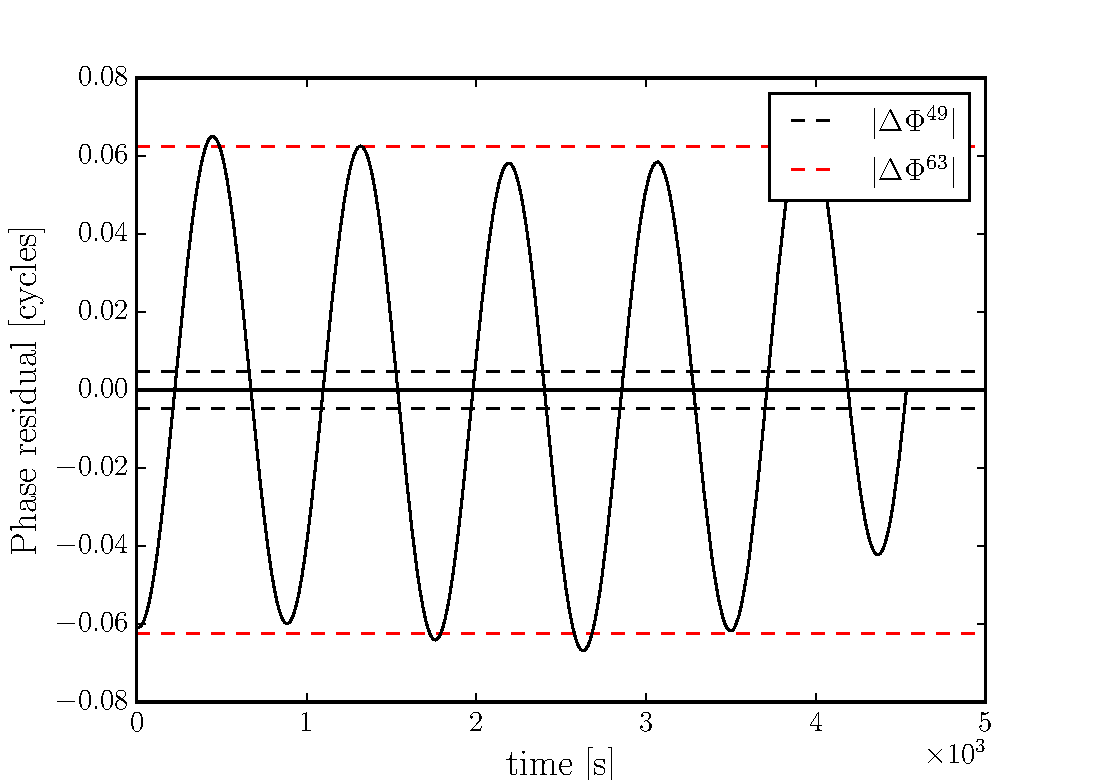
\includegraphics[width=0.7\textwidth]{63_verification.pdf}
%\caption{The phase residual in cycles for a simulated NS with the properties described in table \ref{tab: 49
%verification properties}. This is used to illustrate the agreement with the magnitude
%of variations from equation \eqref{eqn: Jones 49} taken from \citet{Jones2001}.}
%\label{fig: TR 63}
%\end{figure}

\begin{figure}[htb]
\begin{floatrow}
\ffigbox{%
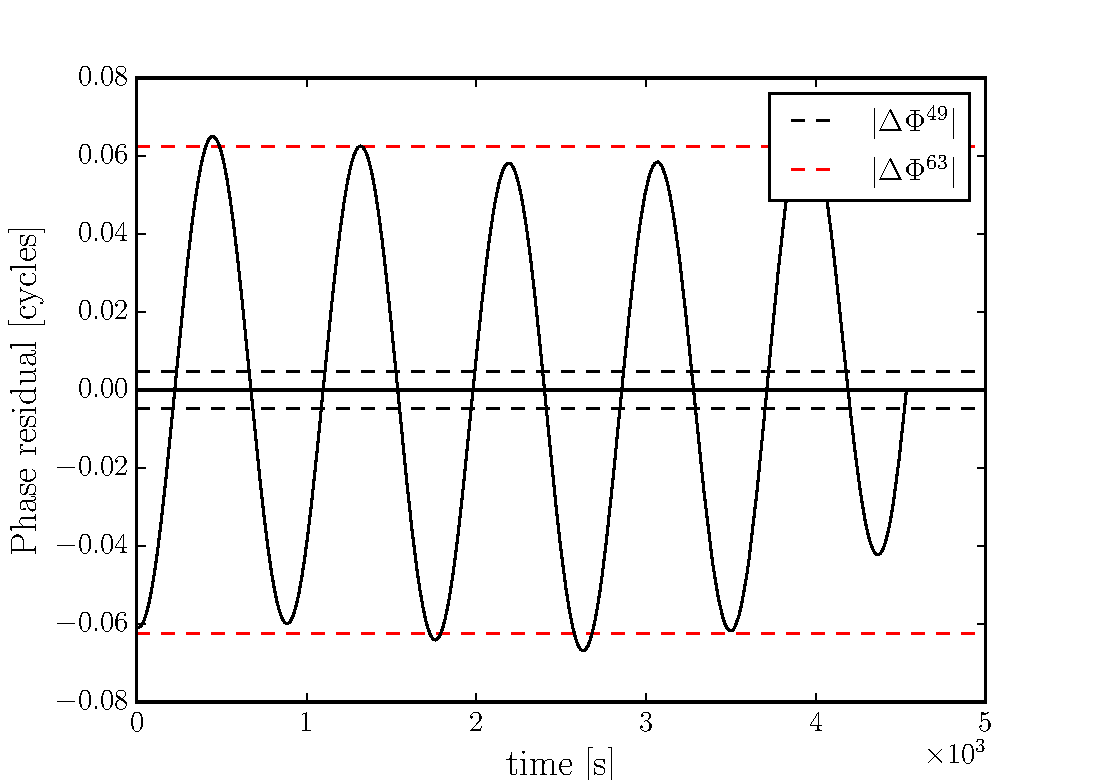
\includegraphics[width=0.5\textwidth]{63_verification.pdf}
}{%
  \caption{The phase residual in cycles for a simulated NS with the properties described in table \ref{tab: 63
verification properties}. This is used to illustrate the agreement with the magnitude
of variations from equation \eqref{eqn: Jones 63} taken from \citet{Jones2001}.}%
  \label{fig: PR 63}
}
\capbtabbox{%
   \begin{tabular}{ccl}
\multicolumn{3}{c}{Simulation parameters} \\
\hline
$\omega_0$  &=& 1550.0 rad/s\\
$B_0$  &=& $ 1.581\times 10^{14} $ G \\
$\chi$  &=& 49.99$^{\circ}$ \\
$a_0$ &=& 2.00$^{\circ}$ \\
$\tilde{\theta}$ &= & 2.06$^{\circ}$ \\
$\mathcal{A}_{\mathrm{EM}}$ &= & $41.0$
\end{tabular}
    
}{%
  \caption{}%
  \label{tab: 63 verification properties}
}
\end{floatrow}
\end{figure}

%In figure \ref{fig: TR no torque} we plot the timing residuals as calculated in
%the torque free model for three values of $\chi$. It is worth noting that the
%power law spin down assumes that the star is in fact spinning down; without the
%torque this model can't not spin down. We can however interpret these results
%as the effect of precession on timing residuals in the limit for which the
%variation due to precession is much stronger than the spin down.
%%\begin{figure}[ht]
%%\centering
%%	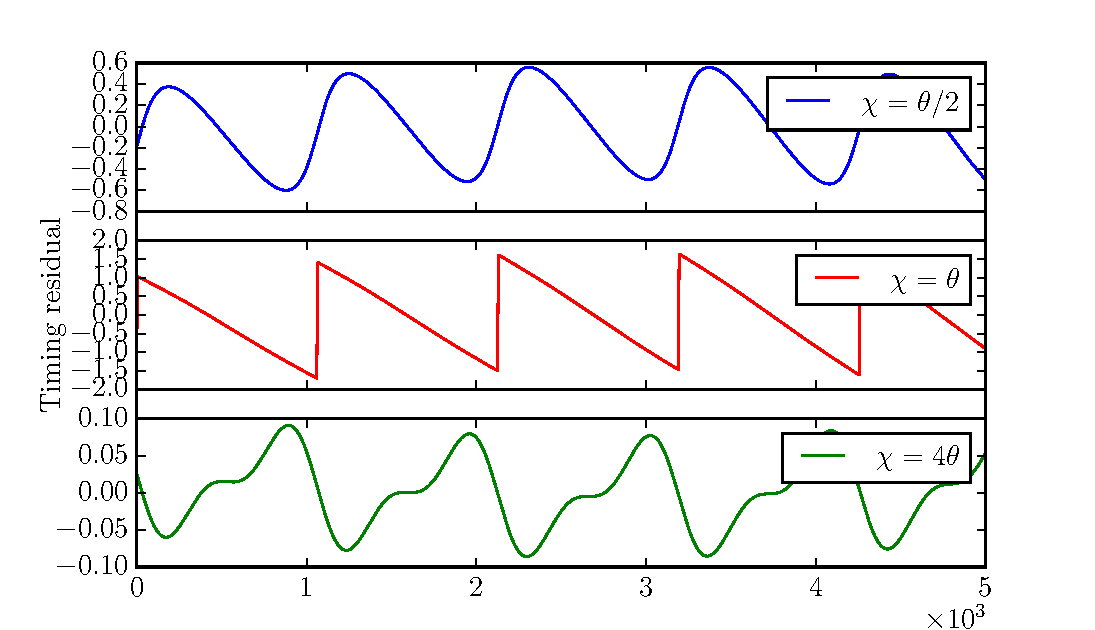
\includegraphics[width=0.7\textwidth]{Timing_residuals_no_torque.pdf}
%%\caption{Plot of the timing residuals for three angles of $\chi$ in the torque
%%         free model showing different types of behaviour. }
%%\label{fig: TR no torque}
%%\end{figure}
%The results show that the precession induces a periodic variation on the
%precession timescale, the magnitude is proportional to the angle $\chi$. We 
%also find the results are dependant on the initial angle $a_{0}$.

\subsection{Effect of free precession on phase residuals: oblique rotator with
electromagnetic torque}

\subsection{Variations in the phase residual due to magnetic dipole inclination}

%\biblio
\end{document}

